\documentclass[sigconf,review]{acmart}

\usepackage{subcaption}
\usepackage{cleveref}

\crefname{figure}{Figure}{Figures}

\acmConference[SPLC'25]{29th International Systems and Software Product Line Conference}{September 01--September 05, 2025}{A Coruña, Spain}

\begin{document}

\title{On digital LEGO product lines for engineering education}

\author{Aleksandra Erohina}
\affiliation{
    \institution{University of Applied Sciences Upper Austria}
    \department{School of Engineering}
    \city{Wels}
    \state{Upper Austria}
    \country{Austria}
}

\author{Georg Hackenberg}
\orcid{0000-0003-3913-4148}
\affiliation{
    \institution{University of Applied Sciences Upper Austria}
    \department{School of Engineering}
    \city{Wels}
    \state{Upper Austria}
    \country{Austria}
}
\email{georg.hackenberg@fh-ooe.at}

\begin{abstract}

    In this paper, we explore the application of software product line engineering (SPLE) principles to the development of physical products, specifically using digital LEGO as a case study. 
    By translating key concepts from the SPLE community, we demonstrate how modularity, variability management, and systematic reuse can enhance the design and production of physical products. 
    Our experience highlights the benefits and challenges of this interdisciplinary approach, providing valuable insights for both software engineers and product designers.

\end{abstract}

\keywords{LEGO}

\maketitle

\section{Introduction}
\label{sec:introduction}

TODO~\cite{Hackenberg_2023} TODO~\cite{Baldwin_2023}

\paragraph{Research objective}

TODO

\paragraph{Research question}

Can we use digital LEGO for building interesting use cases for product line engineering that work well in engineering education?
Can we see typical issues in product line engineering such as module incompatibility in these use cases?
Can we use existing tools for digital LEGO modeling to build up relevant use cases already today?

\paragraph{Contribution}

TODO

\section{Related work}
\label{sec:related-work}

The research begins by conducting a literature review on various topics. 
Firstly, the review focuses on modularity, followed by an exploration of product line engineering.


\subsection{Product line engineering in software domain}
\label{sec:product line engineering}


Product line is a set of products and/or services sharing explicitly defined and managed common and variable features and relying on the same domain architecture to meet the common and variable needs of specific markets.
A concrete product of a product line is called a product variant.

Van der Linden formulated several principles that are fundamental in product line engineering. 
They include, among others, the principle of the two-life-cycle approach, which includes the domain engineering and the application engineering lifecycle, and the principle of variability management.
Domain engineering a reuse-based approach to defining the scope (i.e., domain definition), specifying the structure (i.e., domain architecture), and building the assets (e.g. requirements, designs, software code, documentation) for a class of systems, subsystems, or member products.
During domain analysis, developers determine the scope of the software product line and identify its common and variable features, which they then document in a variability model.
As an example of a variability model, the orthogonal variability model (OVM), introduced by Pohl et al., is used in the next section to manage variability of a drone product line. 

Application engineering is the process of deriving a single variant tailored to the requirements of a specific customer from a product line, based on the results of domain engineering. 
However, with the appearance of second-generation product line engineering, application engineering shrinks to almost nothing; products are produced through the use of high-end industrial strength automation that configures the shared assets appropriately for each product.
Product line engineering goes hand in hand with the concept of modularity.
Li et al. explains modularity as a systematic process where a product or system is composed of various modules, and these modules can be combined in different ways which become different products.
However, clear rules should be set up to reassure that all subsystems will fit and function together in the final design.
The rules are referred among other things to the module interfaces which define how the interacting modules are connected.

\subsection{Product line engineering for the development of physical products}
\label{sec:modualarity}



% Interfaces may involve geometric connections between two components or may involve non-contact interactions. An interface specification defines the mating geometry in cases where there is a geometric connection.
% A connection provides a constraint condition at the contact point of the mechanical unit to guarantee the required function of the composition of parts.
% Constraints limit the range of possible solutions.
% Overall, the interfaces determine the possible configurations, flexibility in use, and number of variants. 



\section{Case study}
\label{sec:case-study}

In this third chapter we introduce the case study, which we have prepared for testing the viability of digital LEGO for product line engineering education.
In the following, we first provide an overview of the selected product line and its product variants in Section~\ref{sec:product-variants}.
Then, we introduce the atomic modules of the product line, from with the individual variants have been assembled in Section~\ref{sec:atomic-modules}.
Finally, we explain the configuration options of the drone use case in the form of a feature tree model in Section~\ref{sec:configuration-options}.

\subsection{Product variants}
\label{sec:product-variants}

\cref{fig:product-variants} provides an overview of the product variants for the drone use case.
The use case comprises three product variants, an ultra-light drone (see \cref{fig:ultra-light}), a free-style drone (see \cref{fig:free-style}), and a long-range drone (see \cref{fig:long-range}).

\begin{description}
    \item[Ultralight drones] designed to comply with regulations by being exceptionally lightweight and compact.
    \item[Freestyle drones] optimized for agility, maneuverability, and creative flight in open environments with a focus on durability for performing aerial acrobatics and complex maneuvers.
    \item[Long-range drones] built for extended flight distances, featuring stable flight characteristics and efficient power consumption.
\end{description}

% \begin{figure*}[htbp]
%     \subcaptionbox{Ultra-light variant\label{fig:ultra-light}}{
%         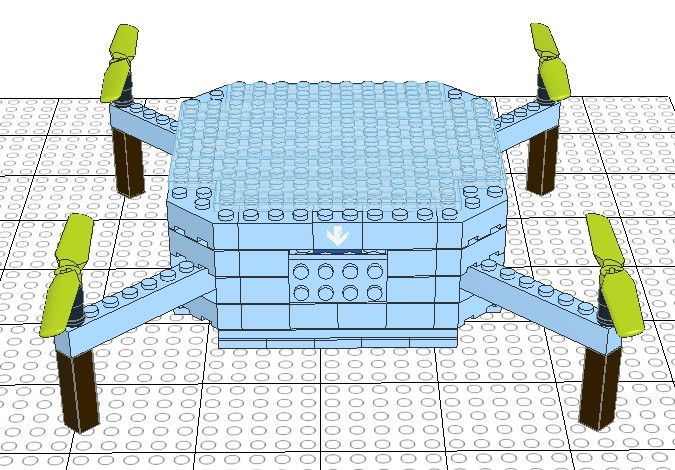
\includegraphics[height=3.1cm]{./UltralightVariant.jpg}
%     }
%     \hfill
%     \subcaptionbox{Free-style variant\label{fig:free-style}}{
%         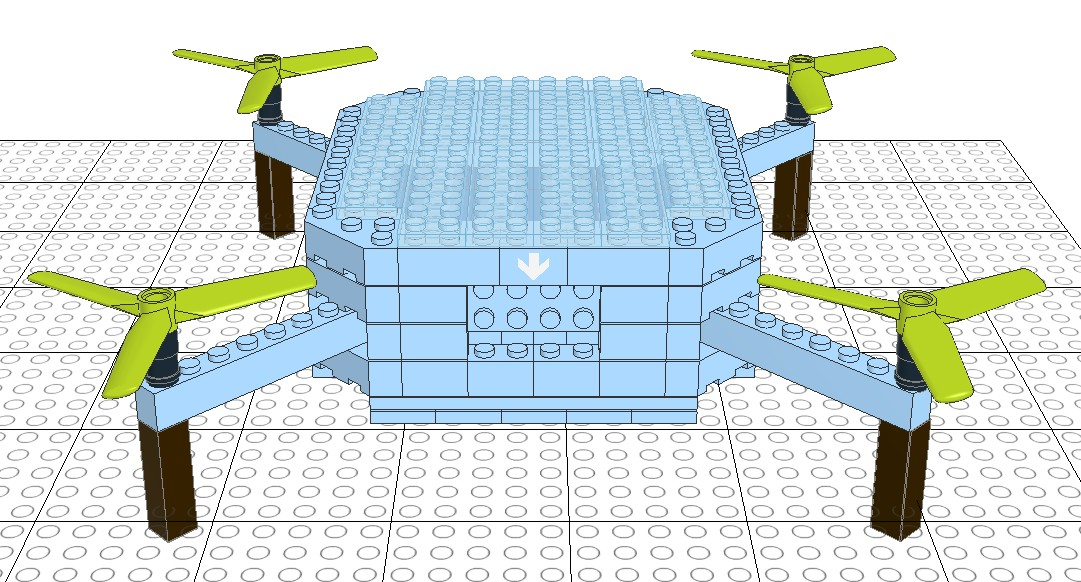
\includegraphics[height=3.1cm]{./FreestyleVariant.jpg}
%     }
%     \hfill
%     \subcaptionbox{Long-range variant\label{fig:long-range}}{
%         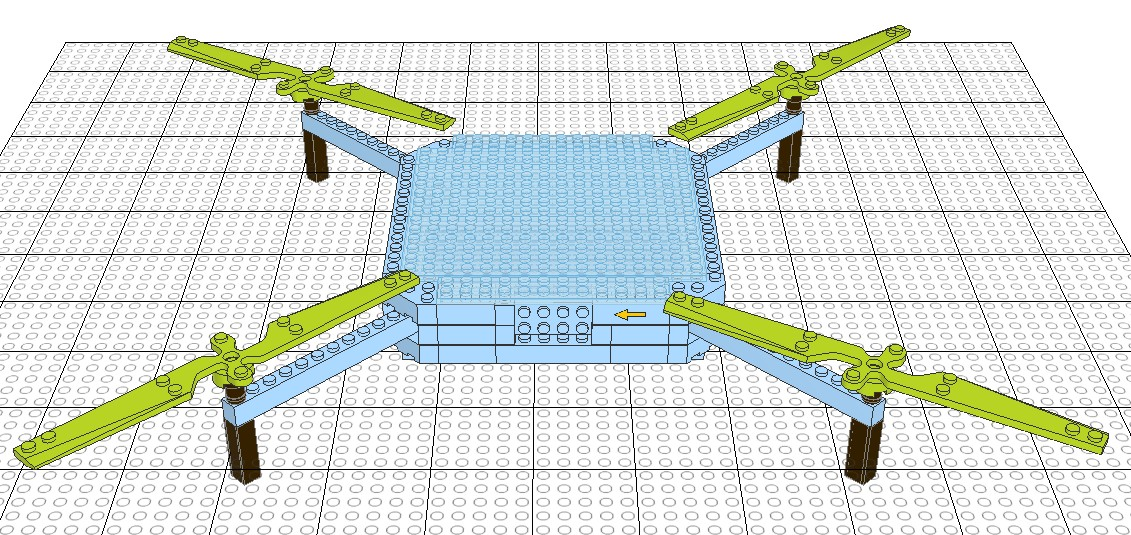
\includegraphics[height=3.1cm]{./LongRangeVariant.jpg}
%     }
%     \caption{Overview of the product variants for the drone use case.}
%     \label{fig:product-variants}
% \end{figure*}

\subsection{Atomic modules}
\label{sec:atomic-modules}

Each drone is made up of four modules, that deliver a certain function. 
Each module has its own variants, which makes it possible to offer a greater variety of products. 

% \begin{figure*}[htbp]
%     \subcaptionbox{Small frame\label{fig:frame-small}}{
%         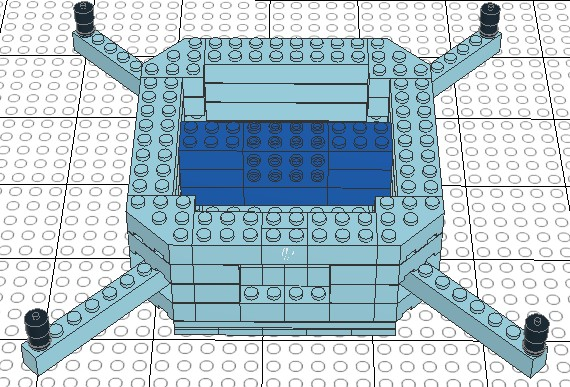
\includegraphics[height=2.3cm]{./drone-case-modules-frame-small.jpg}
%     }
%     \hfill
%     \subcaptionbox{Large frame\label{fig:frame-large}}{
%         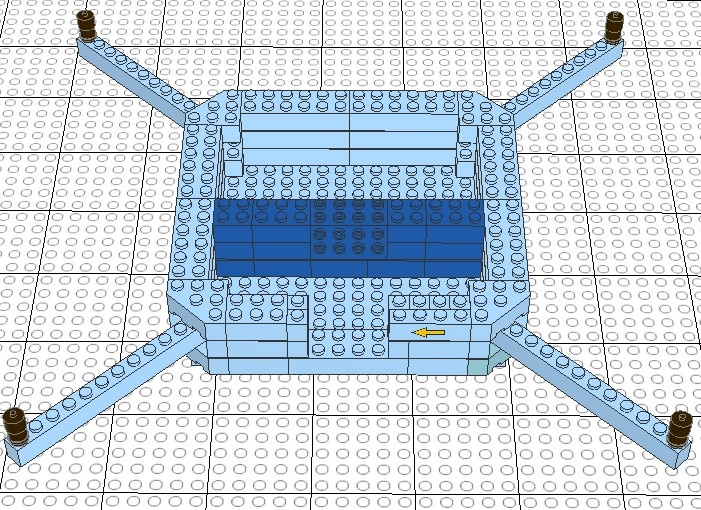
\includegraphics[height=2.3cm]{./drone-case-modules-frame-large.jpg}
%     }
%     \hfill
%     \subcaptionbox{Small battery\label{fig:battery-small}}{
%         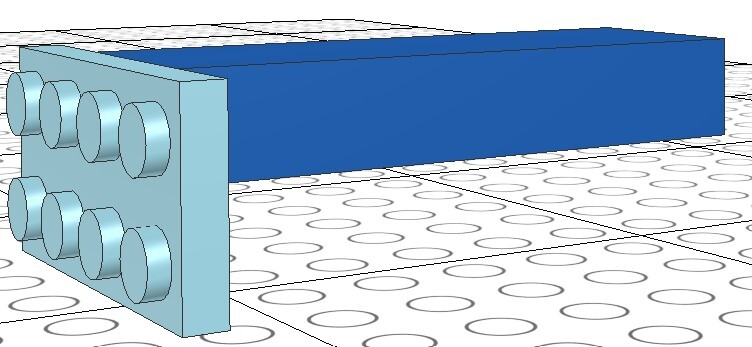
\includegraphics[height=1.3cm]{./drone-case-modules-battery-small.jpg}
%     }
%     \hfill
%     \subcaptionbox{Medium battery\label{fig:battery-medium}}{
%         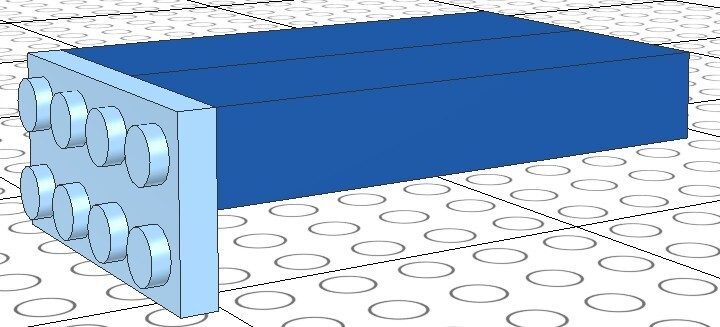
\includegraphics[height=1.3cm]{./drone-case-modules-battery-medium.jpg}
%     }
%     \hfill
%     \subcaptionbox{Large battery\label{fig:battery-large}}{
%         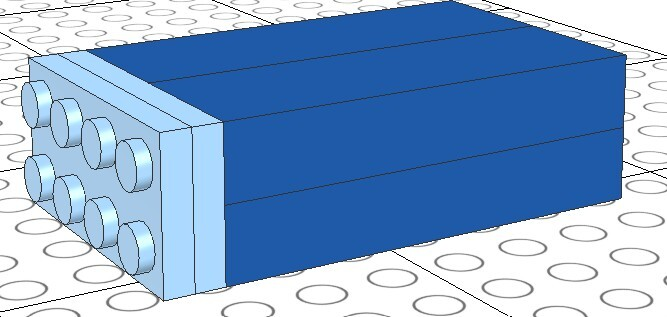
\includegraphics[height=1.3cm]{./drone-case-modules-battery-large.jpg}
%     } 
%     \subcaptionbox{Small cover\label{fig:cover-small}}{
%         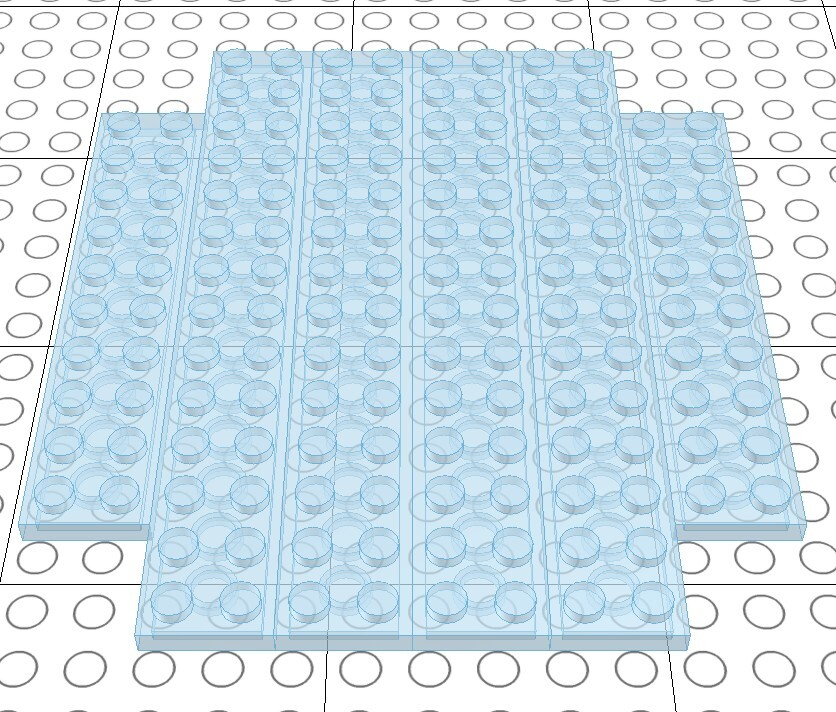
\includegraphics[height=2.3cm]{./drone-case-modules-cover-small.jpg}
%     }
%     \hfill
%     \subcaptionbox{Large cover\label{fig:cover-large}}{
%         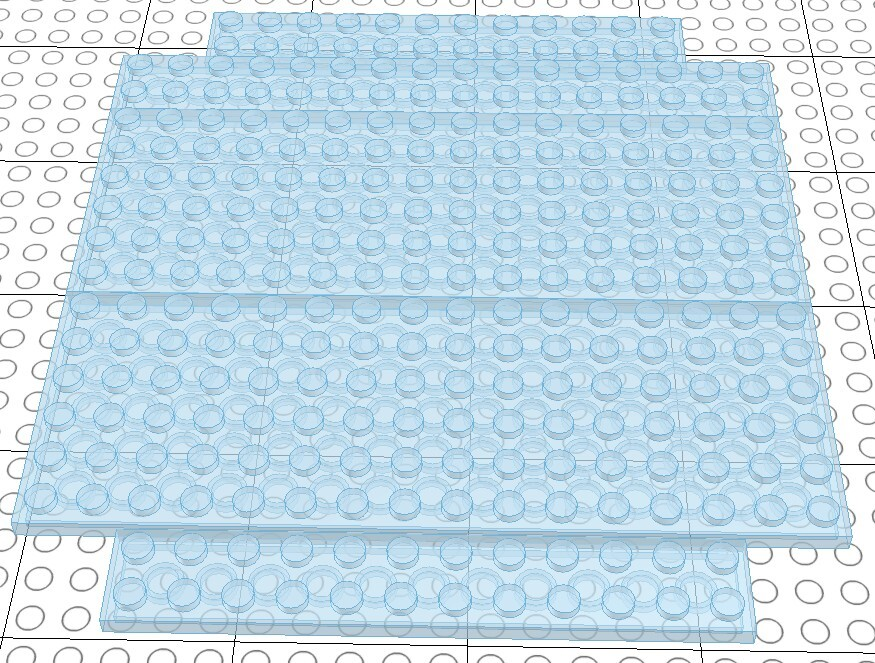
\includegraphics[height=2.3cm]{./drone-case-modules-cover-large.jpg}
%     }
%     \hfill
%     \subcaptionbox{Small propellor\label{fig:propellor-small}}{
%         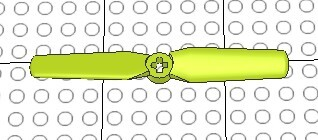
\includegraphics[height=1.5cm]{./drone-case-modules-propellor-2-small.jpg}
%     }
%     \hfill
%     \subcaptionbox{Medium propellor\label{fig:propellor-medium}}{
%         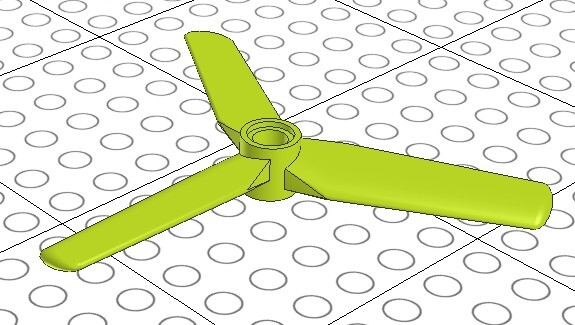
\includegraphics[height=1.5cm]{./drone-case-modules-propellor-3.jpg}
%     }
%     \hfill
%     \subcaptionbox{Large propellor\label{fig:propellor-large}}{
%         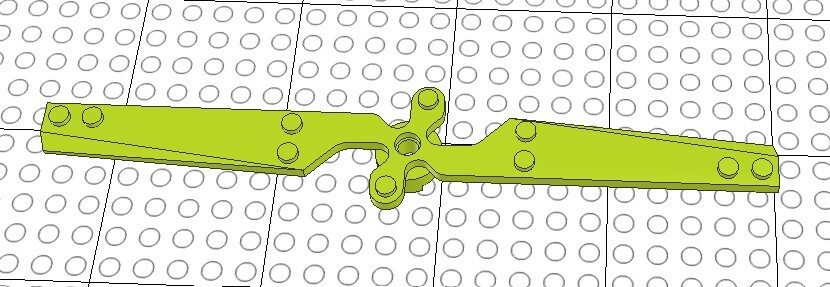
\includegraphics[height=1.5cm]{./drone-case-modules-propellor-2-large.jpg}
%     }

%     \caption{Overview of the atomic modules for the drone use case.}
%     \label{fig:atomic-modules}
% \end{figure*}

\subsubsection{Propellors}
\label{sec:propellors}

Propellers generate thrust by spinning rapidly, allowing a drone to move in all directions. 
A two-blade propeller provides better efficiency and longer flight times, while a triblade propeller offers more stability and maneuverability. 
Smaller propellers provide better agility, while bigger ones provide more thrust and efficiency, allowing the drone fly longer distances. 
However, larger propellers also require more power to spin.

\begin{figure}[htbp]
    \subcaptionbox{Small size\label{fig:propellor-small}}{
        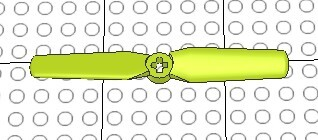
\includegraphics[height=1cm]{./drone-case-modules-propellor-2-small.jpg}
    }
    \hfill
    \subcaptionbox{Medium size\label{fig:propellor-medium}}{
        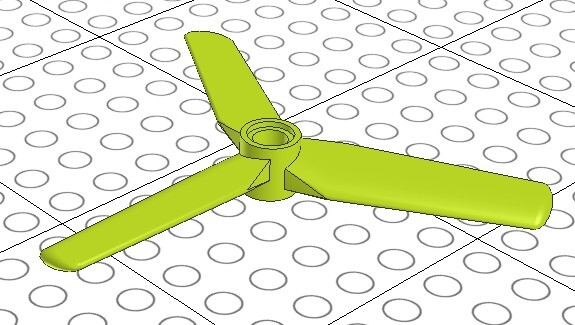
\includegraphics[height=1cm]{./drone-case-modules-propellor-3.jpg}
    }
    \hfill
    \subcaptionbox{Large size\label{fig:propellor-large}}{
        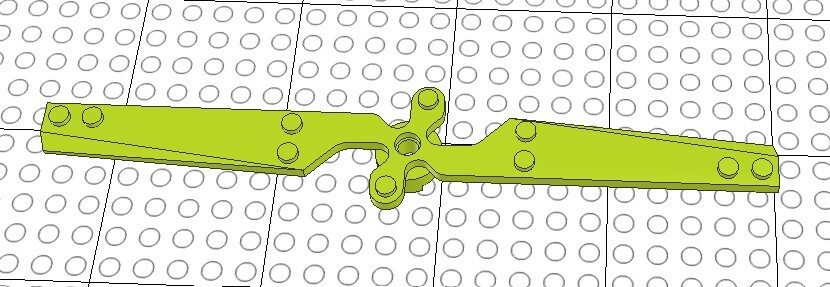
\includegraphics[height=1cm]{./drone-case-modules-propellor-2-large.jpg}
    }
    \caption{Overview of the propeller modules.}
    \label{fig:propeller}
\end{figure}

\subsubsection{Batteries}
\label{sec:batteries}

A battery provides power for the drone to operate. 
A smaller capacity battery is lighter and more compact, which can improve the agility and maneuverability of the drone. 
However, smaller batteries have shorter flight times, which means that for longer flights a higher capacity battery is more suitable.

\begin{figure}[htbp]
    \subcaptionbox{Small size\label{fig:battery-small}}{
        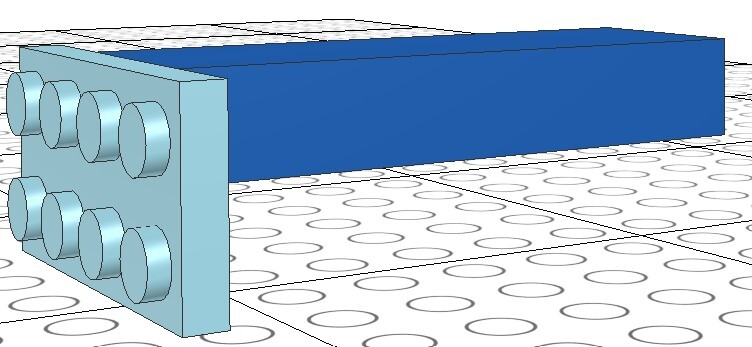
\includegraphics[height=1cm]{./drone-case-modules-battery-small.jpg}
    }
    \hfill
    \subcaptionbox{Medium size\label{fig:battery-medium}}{
        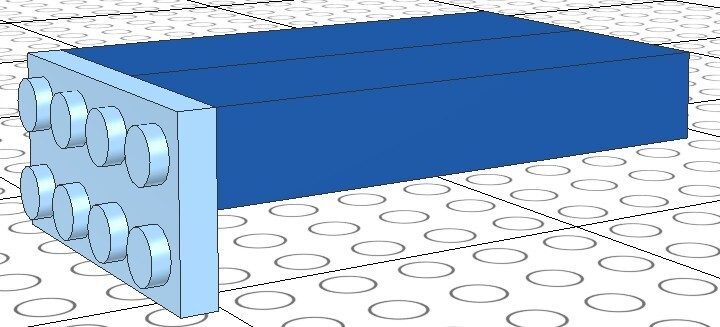
\includegraphics[height=1cm]{./drone-case-modules-battery-medium.jpg}
    }
    \hfill
    \subcaptionbox{Large size\label{fig:battery-large}}{
        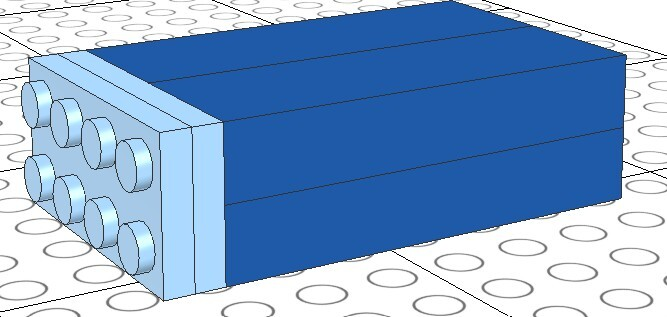
\includegraphics[height=1cm]{./drone-case-modules-battery-large.jpg}
    }
    \caption{Overview of the battery modules.}
    \label{fig:batteries}
\end{figure}

\subsubsection{Frames}
\label{sec:frames}

Frames serve as the structure that holds all the other parts together. 
A small frame is more maneuverable and agile, while a large frame offers more space for additional components (e.g. larger batteries).

\begin{figure}[htbp]
    \subcaptionbox{Small frame\label{fig:frame-small}}{
        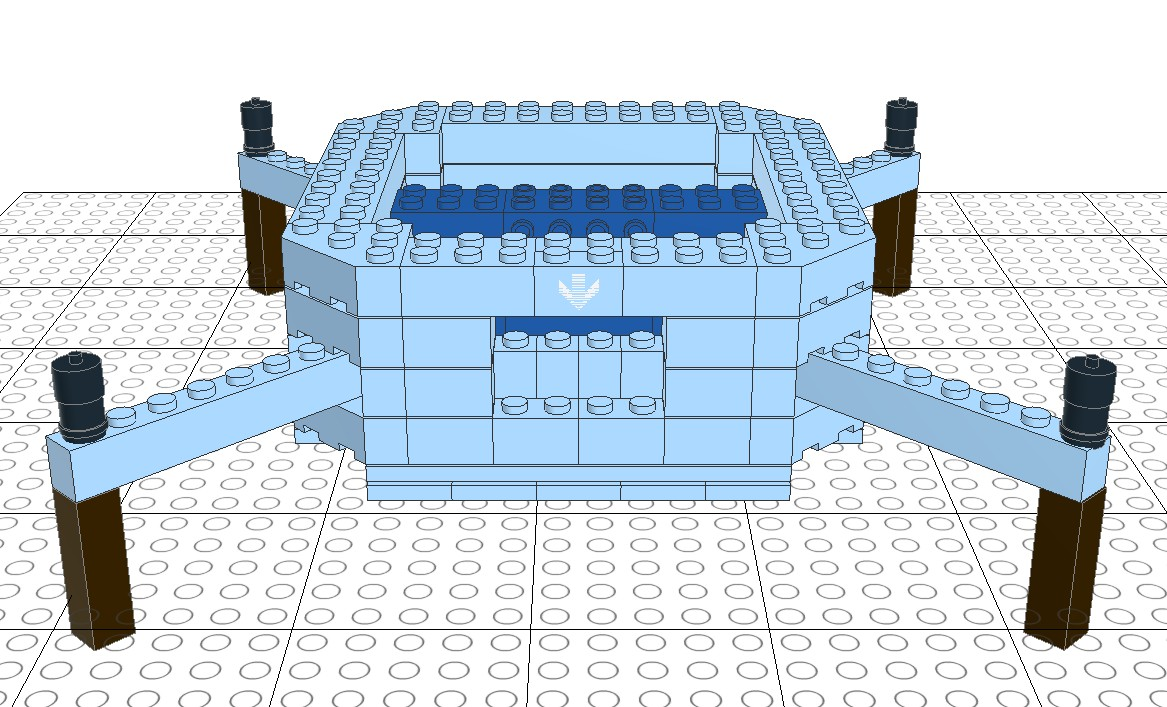
\includegraphics[height=2.1cm]{./SmallFrame.jpg}
    }
    \hfill
    \subcaptionbox{Large frame\label{fig:frame-large}}{
        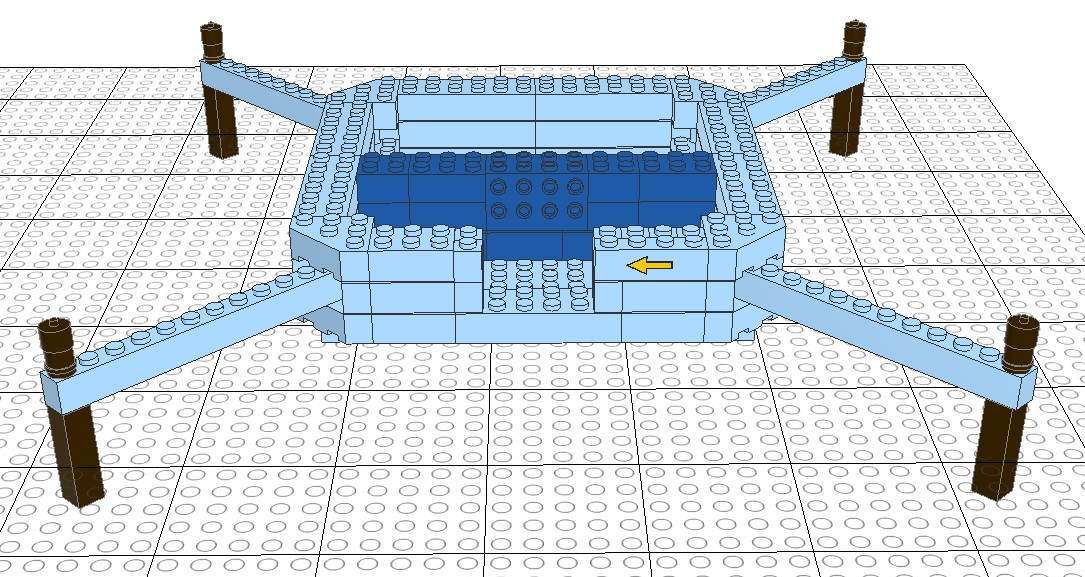
\includegraphics[height=2.1cm]{./LargeFrame.jpg}
    }

    \caption{Overview of the frame modules.}
    \label{fig:frames}
\end{figure}

\subsubsection{Covers}
\label{sec:covers}

Covers protect internal components of the drone, help to improve aerodynamics and serve an aesthetic purpose as well.

\begin{figure}[htbp]
    
    \subcaptionbox{Small cover\label{fig:cover-small}}{
        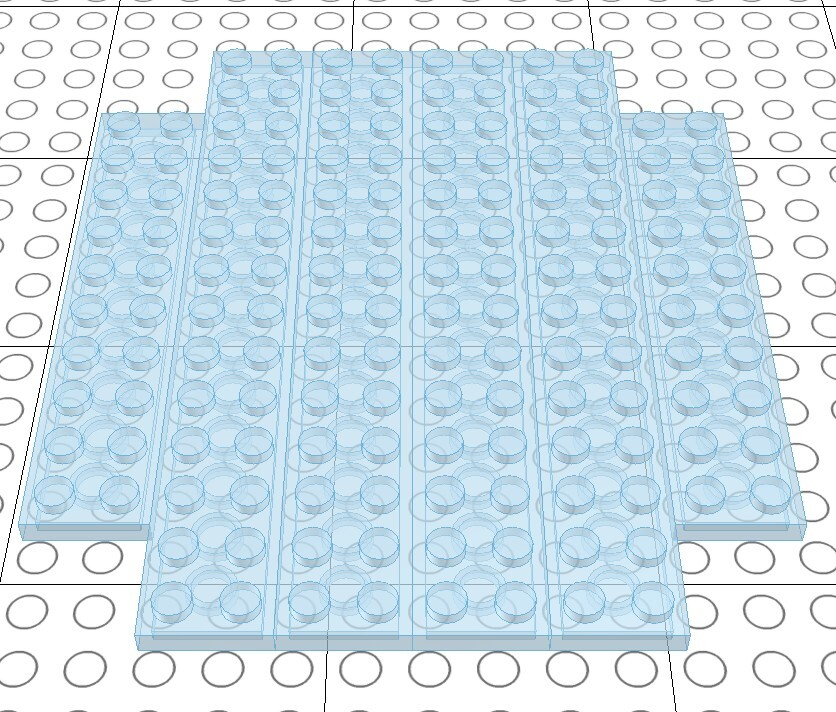
\includegraphics[height=2.1cm]{./drone-case-modules-cover-small.jpg}
    }
    \hfill
    \subcaptionbox{Large cover\label{fig:cover-large}}{
        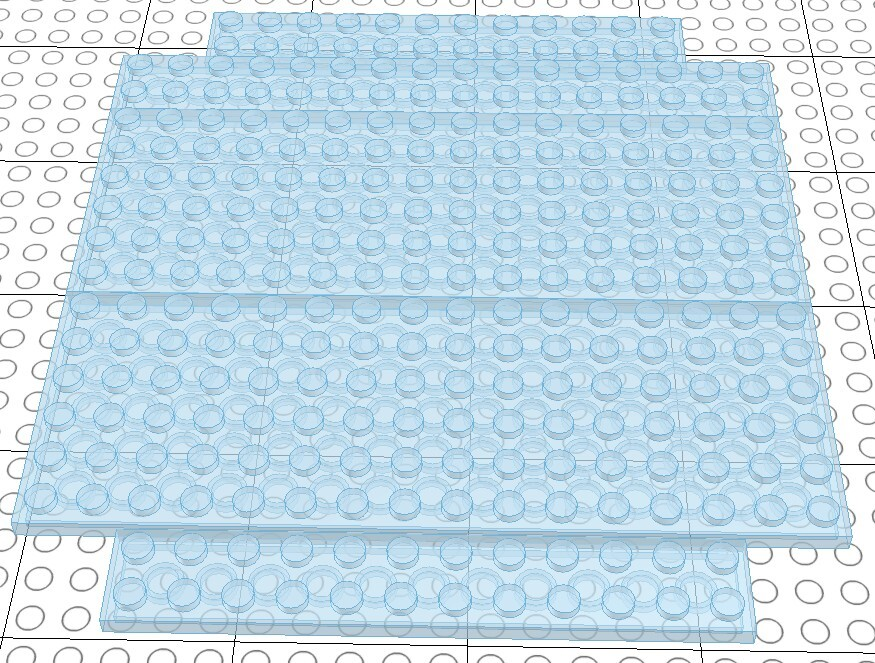
\includegraphics[height=2.1cm]{./drone-case-modules-cover-large.jpg}
    }
    \caption{Overview of the cover modules.}
    \label{fig:atomic-modules}
\end{figure}

\subsection{Configuration options}
\label{sec:configuration-options}

TODO \cref{fig:feature-tree}

\begin{figure*}[htbp]
    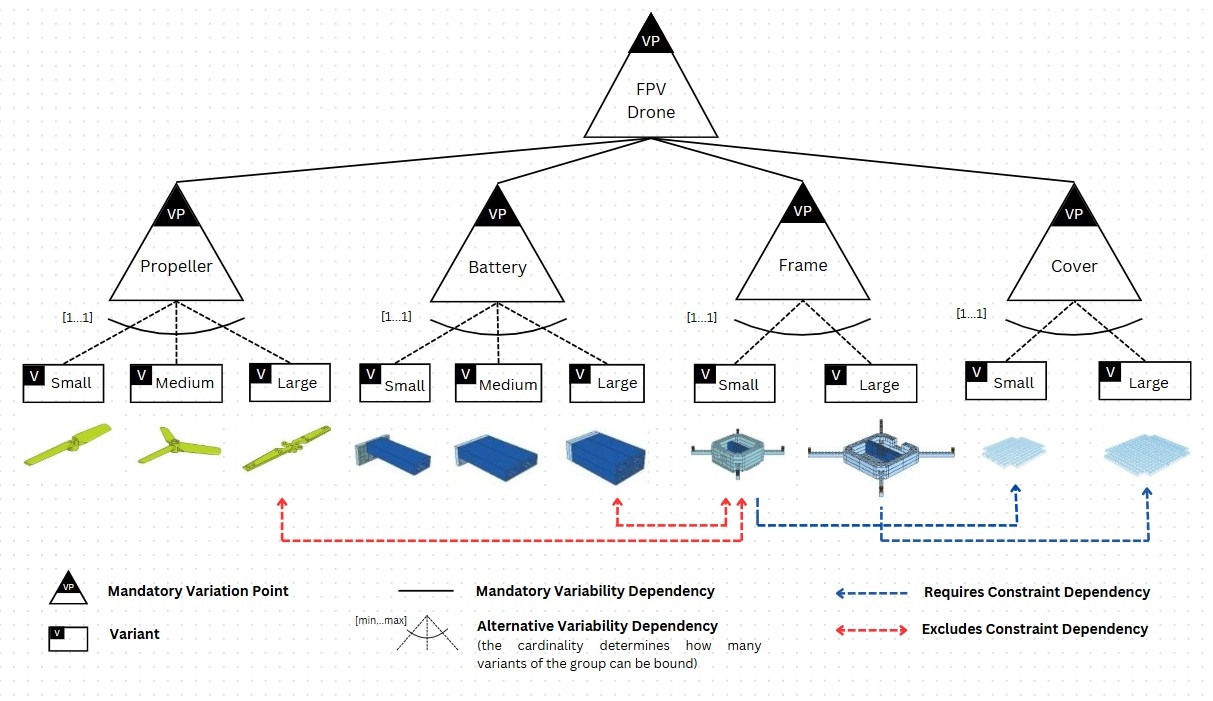
\includegraphics[width=\textwidth]{./FeatureTreeWithLegend3.jpg}
    \caption{Overview of the configuration options for the drone use case.}
    \label{fig:feature-tree}
\end{figure*}

The modules can be combined to design customized end products.  For that purpose, the FPV drone variability model is developed. 
When a customer wishes to design and buy a drone, multiple decisions have to be made before the final system can be build. 
Figure 3 shows that the variation points Propeller, Battery, Frame and Cover have a mandatory dependency with the FPV drone, which means that they have to be included in the final product. 
For each of these variation points a variant has to be selected. The variants are connected by an alternative choice dependency with a minimum and maximum equal to one, which means that only one variant has to be chosen to be included to the final product. 
Additionally, two types of constraint dependencies exist: require constraint and exclude constraint. The require constraint means that when the small frame is selected, the small cover should be integrated to the system, and when the large frame is selected, the large cover should be integrated. 
The excluding constraint means that when a large propeller is selected, the small frame can not be integrated to the design and this relationship goes the other way round as well.

\subsubsection{Interface constraints}

Physical interfaces between interacting modules enable their geometric connection. A frame for the drone example has three interfaces: with a battery, with propellers and with a cover. 
However, several geometrical constraints should be considered. These include:

\begin{description}
    \item[Size and shape constraints] Modules must be designed in such a way that they can physically fit together without interference. 
For the drone example, the large frame can accommodate all three types of batteries, while the small frame is limited to only small and medium batteries because of the size constraints.
    \item[Alignment constraints] Modules must be aligned properly to ensure proper functioning when assembled together. 
For example, covers must be oriented correctly relative to frames to serve the protective and aesthetic purposes. 
    \item[Interference constraints] It is important to consider potential interferences between modules, such as conflicting shapes or components that may impede proper assembly or operation. 
It is technically feasible to install any propeller on any frame, but practical constraints come into play. For instance, a large propeller cannot be mounted on a small frame without interference, as it would collide with the frame during rotation.
These geometric restrictions cause constraint dependencies that are shown in Figure 3.
\end{description}

\subsection{150\% model}
\label{sec:150-model}

The case study demonstrates the utilization of digital LEGOs to create a 150\% model of a 3D drone architecture. 
This model is build in LeoCAD, a program that adheres to the LDraw standard. 
Within the structure of the LDraw file, a main document serves as the foundation where all three variants of the drone are instantiated. 
Each variant is further segmented into submodels, which consist of modular components. 
These modules are essentially instances of the submodels, all organized within the same file.

The approach enables to reuse the modules and submodels, promoting efficiency and versatility in design. 
The 150\% model encompasses all feasible combinations of drone features across the different variants. 
This abundance of information extends beyond the actual requirements of a specific drone type; for instance, showcasing three distinct battery sizes even though a practical FPV drone would only utilize one.


\begin{figure*}[htbp]
    \includegraphics[width=\textwidth]{./150_MODEL_6.jpg}
    \caption{Overview of the 150\% model for the drone use case.}
    \label{fig:150-model}
\end{figure*}

TODO

\section{Conclusion}
\label{sec:conclusion}

TODO

\bibliography{main}
\bibliographystyle{ACM-Reference-Format}

\end{document}